\documentclass[dutch]{ucll-slides}
\usepackage{pxfonts}
\usepackage{tikz}
\usepackage{calc}
\usepackage{fmtcount}
\usepackage{bbding}


\usetikzlibrary{calc,shadows,math}

\title{Programmeertalen}

\newcommand{\csharp}{C$^\sharp$}
\newcommand{\cpp}{C++}
\newcommand{\pro}{\Checkmark}
\newcommand{\con}{\XSolidBrush}


\newcounter{dummy}

\tikzset{
  /tikz/.cd,
  language/.style={drop shadow,fill=blue!50,font=\scshape,minimum height=.75cm,minimum width=1.5cm}
}


\begin{document}

\maketitle

\section{Programmeertalen}

\begin{frame}
  \frametitle{Programmeertalen}
  \begin{center}
    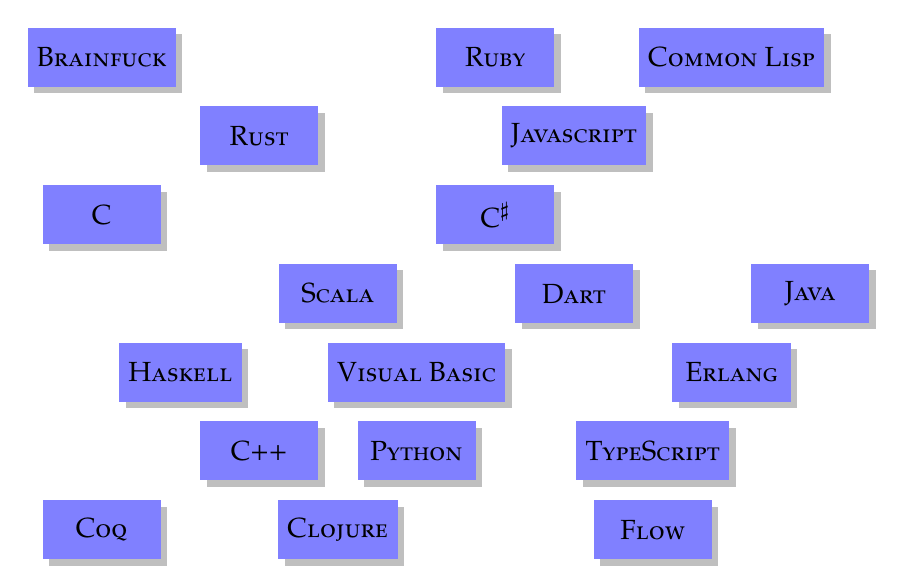
\begin{tikzpicture}
      \node[language] at (5,1) {Java};
      \node[language] at (2,3) {Javascript};
      \node[language] at (1,2) {\csharp};
      \node[language] at (-2,-1) {\cpp};
      \node[language] at (-4,2) {C};
      \node[language] at (0,-1) {Python};
      \node[language] at (1,4) {Ruby};
      \node[language] at (-2,3) {Rust};
      \node[language] at (-4,-2) {Coq};
      \node[language] at (3,-1) {TypeScript};
      \node[language] at (3,-2) {Flow};
      \node[language] at (4,0) {Erlang};
      \node[language] at (-1,1) {Scala};
      \node[language] at (-1,-2) {Clojure};
      \node[language] at (-3,0) {Haskell};
      \node[language] at (2,1) {Dart};
      \node[language] at (4,4) {Common Lisp};
      \node[language] at (-4,4) {Brainfuck};
      \node[language] at (0,0) {Visual Basic};
    \end{tikzpicture}
  \end{center}
\end{frame}

\begin{frame}
  \frametitle{Programmeertalen}
  \begin{itemize}
    \item Veel programmeertalen (duizenden)
    \item Waarom bestaan ze?
    \item Hoe verschillen ze van elkaar?
    \item Is het nuttig om er meerdere te kennen?
    \item Welke zien we in de opleiding?
  \end{itemize}
\end{frame}

\subsection{Wat is Programmeren?}

\begin{frame}
  \tableofcontents[currentsubsection]
\end{frame}

\begin{frame}
  \frametitle{Wat is Programmeren?}
  \begin{center}
    Programmeren is \\
    machine vertellen hoe reageren op inputs
  \end{center}
  \vskip5mm
  \begin{center}
    \begin{tikzpicture}[box/.style={minimum width=3cm,minimum height=1cm,draw,fill=blue!50,drop shadow},scale=0.8,transform shape]
      \node[box] (pc) {Computer};
      \node[box] (mouse) at (150:5) {Muis};
      \node[box] (keyboard) at (210:5) {Toetsenbord};
      \node[box] (screen) at (30:5) {Scherm};
      \node[box] (speakers) at (-30:5) {Speakers};

      \only<2-3>{
        \draw[-latex] (keyboard) -- (pc) node[below,midway,sloped,font=\tiny] {S ingedrukt};

        \only<3>{
          \draw[-latex] (pc) -- (screen) node[below,midway,sloped,font=\tiny] {toon S};
        }
      }

      \only<4-5>{
        \draw[-latex] (mouse) -- (pc) node[below,midway,sloped,font=\tiny] {klik op knop};

        \only<5>{
          \draw[-latex] (pc) -- (speakers) node[below,midway,sloped,font=\tiny] {klikgeluid};
          \draw[-latex] (pc) -- (screen) node[below,midway,sloped,font=\tiny] {toon ingedrukte knop};
        }
      }
    \end{tikzpicture}
  \end{center}
\end{frame}

\subsection{Waarom Bestaan Programmeertalen?}

\begin{frame}
  \tableofcontents[currentsubsection]
\end{frame}

\begin{frame}
  \frametitle{Waarom Bestaan Programmeertalen?}
  \begin{center}
    Time flies like an arrow \\
    Fruit flies like a banana \\[4mm]
    Plus de pain! \\[4mm]
    Veel diarree\kern1pt gevallen in Nickerie
  \end{center}
\end{frame}

\begin{frame}
  \frametitle{Waarom Bestaan Programmeertalen?}
  \begin{itemize}
    \item Spreektalen zijn vaak dubbelzinnig
    \item We kiezen onbewust voor de meest logische interpretatie
    \item Machines hebben geen ``common sense''
    \item Machine moet \emph{exacte} instructies ontvangen
    \item Programmeertalen zijn veel strikter en nauwkeuriger
  \end{itemize}
\end{frame}

\subsection{Hoe Werkt Programmeren?}

\begin{frame}
  \tableofcontents[currentsubsection]
\end{frame}

\begin{frame}
  \frametitle{Hoe Werkt Programmeren?}
  \begin{itemize}
    \item Taal biedt basisbouwblokken
    \item Taal biedt mogelijkheid om bouwblokken te combineren
    \item Zo ontstaan nieuwe bouwblokken (\emph{abstracties})
  \end{itemize}
\end{frame}

\begin{frame}
  \frametitle{Voorbeeld}
  \begin{center}
    \begin{tikzpicture}
      \draw (-5,-3) rectangle (5,3);
      \only<1>{
        \node {\ttfamily 0};
      }
      \only<2>{
        \node {\ttfamily 11001011};
      }
      \only<3>{
        \node[draw] {\ttfamily
          \begin{tabular}{c}
            10010101 \\
            10100110 \\
            01001010 \\
          \end{tabular}
        };
      }
      \only<4>{
        \begin{scope}[scale=0.4,transform shape]
          \foreach \x in {-10,-8,...,10} {
            \foreach \y in {-6,-4.5,...,6} {
              \node[draw,inner sep=2pt,font=\small] at (\x,\y) {\ttfamily%
                \tikzmath{
                  int \a;
                  int \b;
                  int \c;
                  \a = random(255);
                  \b = random(255);
                  \c = random(255);
                }%
                \parbox{1.5cm}{\centering%
                  {\setcounter{dummy}{\a}\padzeroes[8]{\binary{dummy}}} \\
                  {\setcounter{dummy}{\b}\padzeroes[8]{\binary{dummy}}} \\
                  {\setcounter{dummy}{\c}\padzeroes[8]{\binary{dummy}}}
                }
              };
            }
          }
        \end{scope}
      }
    \end{tikzpicture}
  \end{center}
  \begin{overprint}
    \onslide<1>
    \begin{center}
      Bit als eenvoudigste bouwblok
    \end{center}

    \onslide<2>
    \begin{center}
      Met 8 bits bouwen we een getal
    \end{center}

    \onslide<3>
    \begin{center}
      Drie getallen vormen samen een kleur
    \end{center}

    \onslide<4>
    \begin{center}
      Een tabel kleuren vormt een beeld
    \end{center}
  \end{overprint}
\end{frame}

\begin{frame}
  \frametitle{Abstractietoren}
  \begin{center}
    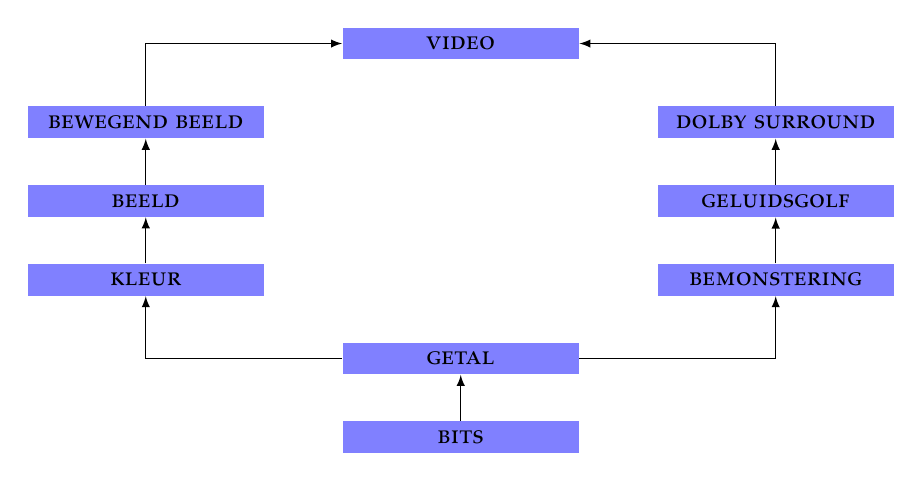
\begin{tikzpicture}[level/.style={fill=blue!50,minimum width=3cm,font=\scshape},
                        link/.style={-latex}]
      \node[level] (bits) at (0,0) {bits};
      \node[level] (number) at (0,1) {getal};
      \node[level] (color) at (-4,2) {kleur};
      \node[level] (image) at (-4,3) {beeld};
      \node[level] (animation) at (-4,4) {bewegend beeld};
      \draw[link] (bits) -- (number);
      \draw[link] (number) -| (color);
      \draw[link] (color) -- (image);
      \draw[link] (image) -- (animation);

      \node[level] (sample) at (4,2) {bemonstering};
      \node[level] (wave) at (4,3) {geluidsgolf};
      \node[level] (sound) at (4,4) {dolby surround};

      \draw[link] (number) -| (sample);
      \draw[link] (sample) -- (wave);
      \draw[link] (wave) -- (sound);

      \node[level] (movie) at (0,5) {video};
      \draw[link] (animation) |- (movie);
      \draw[link] (sound) |- (movie);
    \end{tikzpicture}
  \end{center}
\end{frame}

\subsection{Machinetaal}

\begin{frame}
  \tableofcontents[currentsubsection]
\end{frame}

\begin{frame}
  \frametitle{Moedertaal Machine}
  \begin{itemize}
    \item Verstaat de machine dan zoveel talen? \\[2mm]
    \item Zijn talen misschien machine-afhankelijk?
          \begin{itemize}
            \item Werkt Java enkel op Mac?
            \item Werkt Python enkel op Playstations?
          \end{itemize}
  \end{itemize}
\end{frame}

\begin{frame}
  \frametitle{Moedertaal Machine}
  \begin{itemize}
    \item Een machine verstaat maar \'e\'en taal
    \item Dit is de ``moedertaal'' van die machine
    \item Elke machine heeft eigen moedertaal
    \item Een programma geschreven in een andere taal moet eerst vertaald worden
  \end{itemize}
\end{frame}

\begin{frame}
  \frametitle{Machinetaal}
  \begin{itemize}
    \item Waarom niet rechtstreeks in machinetaal programmeren?
    \item Waarom de moeite doen om andere talen te ontwikkelen?
  \end{itemize}
\end{frame}

\begin{frame}
  \frametitle{Machinetaal}
  \structure{Voorbeeldprogramma}
  \begin{center} \ttfamily
    01101000 01110100 01110100 01110000 \\
    01110011 00111010 00101111 00101111 \\
    01111001 01101111 01110101 01110100 \\
    01110101 00101110 01100010 01100101 \\
    00101111 01110011 01010100 01010011 \\
    01000001 01011111 01110011 01010111 \\
    01000111 01001101 00110100 00110100 
  \end{center}
  \vskip5mm
  \begin{center}
    Nuff said
  \end{center}
\end{frame}

\begin{frame}
  \frametitle{Platformonafhankelijkheid}
  \begin{itemize}
    \item Machinetaal werkt enkel op corresponderende machine
    \item We willen zelfde programma niet meermaals herschrijven
    \item We schrijven het eenmaal en vertalen het meermaals
  \end{itemize}
  \vskip5mm
  \begin{center}
    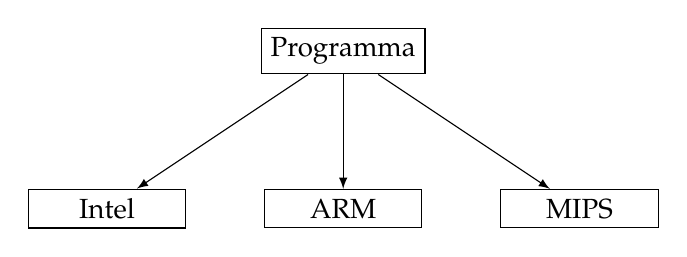
\begin{tikzpicture}[block/.style={draw,minimum width=2cm},
                        translate/.style={-latex}]
      \node[block] (source) at (0,2) {Programma};
      \node[block] (intel) at (-3,0) {Intel};
      \node[block] (arm) at (0,0) {ARM};
      \node[block] (mips) at (3,0) {MIPS};

      \draw[translate] (source) -- (intel);
      \draw[translate] (source) -- (arm);
      \draw[translate] (source) -- (mips);
    \end{tikzpicture}
  \end{center}
\end{frame}



%%% Local Variables:
%%% mode: latex
%%% TeX-master: "programming-languages"
%%% End:

\section{Verschillen Tussen Talen}

\subsection{Turing Completeness}

\begin{frame}
  \tableofcontents[currentsection]
\end{frame}

\begin{frame}
  \frametitle{Turing Completeness}
  \begin{itemize}
    \item Hoe ``krachtig'' is een taal?
    \item Zijn er talen die meer kunnen dan andere?
    \item Kan een programma geschreven in taal X ook geschreven worden in taal Y?
  \end{itemize}
\end{frame}

\begin{frame}
  \frametitle{Turing Completeness}
  \begin{itemize}
    \item Een taal is Turing complete indien elk mogelijk programma erin kan geschreven worden
    \item (Zo goed als) Alle talen zijn Turing complete
    \item M.a.w.~(bijna) alle talen zijn equivalent qua ``kracht''
  \end{itemize}
\end{frame}

\begin{frame}
  \frametitle{Visualisatie}
  \begin{center}
    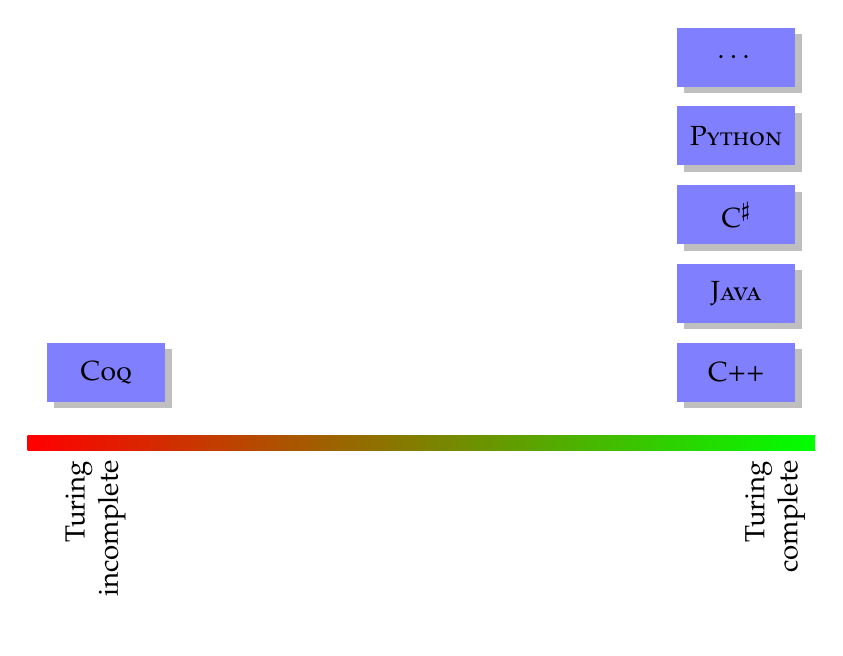
\begin{tikzpicture}
      \shade [left color=red,right color=green] (0,0) rectangle (10,0.2);
      \node[anchor=north east,rotate=90] at (0,0) {\parbox{2cm}{\flushright Turing \\ incomplete}};
      \node[anchor=south east,rotate=90] at (10,0) {\parbox{2cm}{\flushright Turing \\ complete}};

      \node[language] at (9,1) {\cpp};
      \node[language] at (9,2) {Java};
      \node[language] at (9,3) {\csharp};
      \node[language] at (9,4) {Python};
      \node[language] at (9,5) {\dots};
      \node[language] at (1,1) {Coq};
    \end{tikzpicture}
  \end{center}
\end{frame}


\subsection{Effici\"entie}

\begin{frame}
  \tableofcontents[currentsubsection]
\end{frame}

\begin{frame}
  \frametitle{Effici\"entie}
  \begin{itemize}
    \item Sommige talen focussen zuiver op snelheid van uitvoering
    \item Geen poging om veilig te zijn
    \item C/\cpp\ zien snelheid als topprioriteit
  \end{itemize}
  \begin{center}
    \includegraphics[width=5cm]{unsafe-driving.jpg}
  \end{center}
\end{frame}

\begin{frame}
  \frametitle{Effici\"entie}
  \begin{itemize}
    \item Veel talen offeren snelheid op voor veiligheid
    \item Checken constant op mogelijke fouten tijdens uitvoering
    \item Bv.~\csharp, Java
  \end{itemize}
  \begin{center}
    \includegraphics[width=5cm]{drive-safely.jpg}
  \end{center}
\end{frame}

\begin{frame}
  \frametitle{Effici\"entie}
  \begin{itemize}
    \item Andere talen verkiezen comfort en flexibiliteit
    \item Kunnen 100$\times$ trager zijn dan C/C++
    \item Bv.~Ruby, Python, Common Lisp
  \end{itemize}
  \begin{center}
    \includegraphics[width=5cm]{luxury-driving.jpg}
  \end{center}
\end{frame}

\begin{frame}
  \frametitle{Visualisatie}
  \begin{center}
    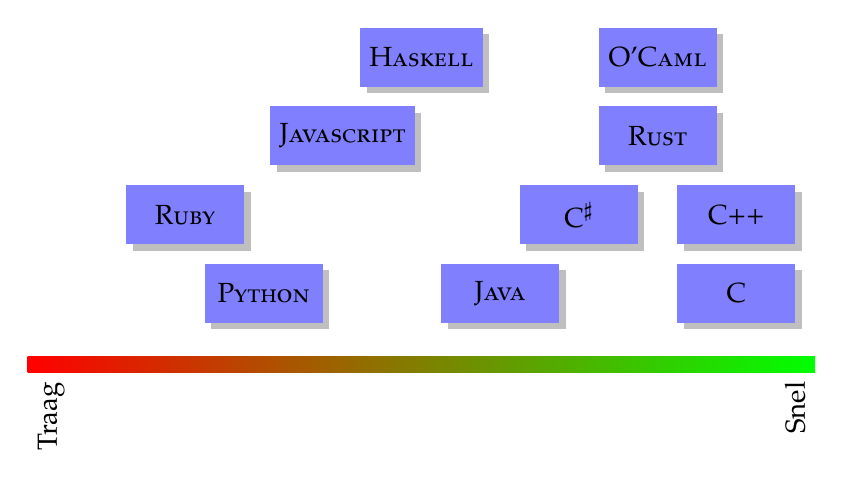
\begin{tikzpicture}
      \shade [left color=red,right color=green] (0,0) rectangle (10,0.2);
      \node[anchor=north east,rotate=90] at (0,0) {Traag};
      \node[anchor=south east,rotate=90] at (10,0) {Snel};

      \node[language] at (9,1) {C};
      \node[language] at (9,2) {\cpp};
      \node[language] at (8,3) {Rust};
      \node[language] at (8,4) {O'Caml};
      \node[language] at (6,1) {Java};
      \node[language] at (7,2) {\csharp};
      \node[language] at (3,1) {Python};
      \node[language] at (4,3) {Javascript};
      \node[language] at (5,4) {Haskell};
      \node[language] at (2,2) {Ruby};
    \end{tikzpicture}
  \end{center}
\end{frame}

\subsection{Bugdetectie}

\begin{frame}
  \tableofcontents[currentsubsection]
\end{frame}

\begin{frame}
  \frametitle{Bugdetectie}
  \begin{itemize}
    \item Schrijven van code is niet eenvoudig
    \item Bugs onvermijdelijk
    \item Hoe kunnen we met bugs omgaan?
  \end{itemize}
\end{frame}

\begin{frame}
  \frametitle{Optie \#1: Bugs Volledig Vermijden}
  \begin{itemize}
    \item Wiskundige analyses loslaten op code
    \item Programma pas uitgeven als 100\%\ correctheid bewezen is
    \item Heet ``compile time checking''
  \end{itemize}
  \vskip4mm
  \structure{Voor- en Nadelen}
  \begin{itemize}
    \item[\pro] Klant krijgt perfect werkend product
    \item[\con] Kost gigantisch veel moeite
          \begin{itemize}
            \item Bv.~taal Coq
            \item Productiviteit 100$\times$ lager
          \end{itemize}
  \end{itemize}
  \vskip4mm
  \structure{In de Praktijk}
  \begin{itemize}
    \item Belangrijk voor ziekenhuissoftware, vliegtuigen, \dots
  \end{itemize}
\end{frame}

\begin{frame}
  \frametitle{Optie \#2: Bugs Detecteren Tijdens Uitvoering}
  \begin{itemize}
    \item Tijdens uitvoering situatie constant monitoren
    \item Indien iets niet klopt: situatie herstellen of alles stopzetten
    \item Heet ``runtime checking''
  \end{itemize}
  \vskip4mm
  \structure{Voor- en Nadelen}
  \begin{itemize}
    \item[\pro] Goedkoper om te ontwikkelen
    \item[\con] Klant krijgt buggy programma
    \item[\con] Programma werkt trager, vergt meer geheugen
  \end{itemize}
\end{frame}

\begin{frame}
  \frametitle{Optie \#3: Bugs Negeren}
  \begin{itemize}
    \item Ervan uitgaan dat er gewoon geen bugs zijn
    \item Indien wel bug: blijven doorgaan
  \end{itemize}
  \vskip4mm
  \structure{Voor- en Nadelen}
  \begin{itemize}
    \item[\pro] Goedkoop om te ontwikkelen
    \item[\pro] Programma draait heel effici\"ent
    \item[\con] Klant krijgt foute resultaten zonder het te beseffen
  \end{itemize}
\end{frame}

\begin{frame}
  \frametitle{Visualisatie}
  \begin{center}
    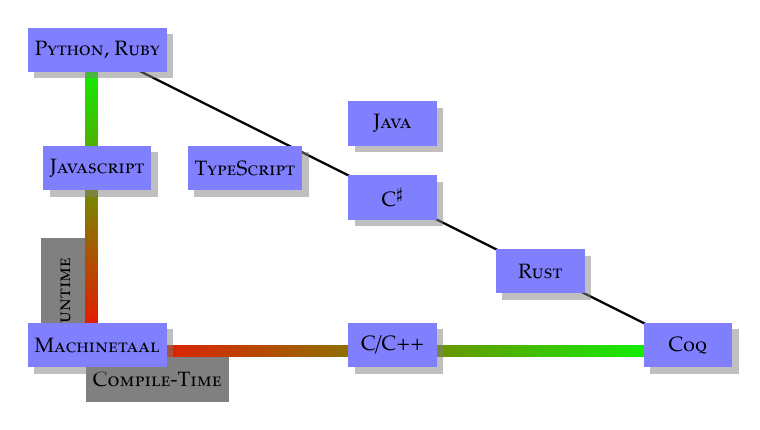
\begin{tikzpicture}[scale=.75,transform shape,
                        header/.style={fill=gray,minimum width=2cm,minimum height=0.75cm,font=\scshape}]
      \shade [left color=red,right color=green] (-0.2,0) rectangle (10,-0.2);
      \shade [left color=red,right color=green,shading angle=180] (0,-0.2) rectangle (-0.2,5);
      \draw[thick] (0,5) -- (10,0);
      
      \node[header,anchor=north west] at (-0.2,-0.2) {Compile-Time};
      \node[header,anchor=south west,rotate=90] at (-0.2,-0.2) {Runtime};

      \node[language] at (5,0) {C/\cpp};
      \node[language] at (7.5,1.25) {Rust};
      \node[language] at (10,0) {Coq};
      \node[language] at (5,3.75) {Java};
      \node[language] at (5,2.5) {\csharp};
      \node[language] at (2.5,3) {TypeScript};
      \node[language] at (0,3) {Javascript};
      \node[language] at (0,5) {Python, Ruby};
      \node[language] at (0,0) {Machinetaal};
    \end{tikzpicture}
  \end{center}

  \begin{overprint}
    \onslide<1>
    \begin{center}
      De meeste talen combineren compile-time met runtime checks \\ (bv. \csharp, Java, TypeScript, Rust)
    \end{center}

    \onslide<2>
    \begin{center}
      Python, Ruby en Javascript voeren enkel checks uit at runtime
    \end{center}

    \onslide<3>
    \begin{center}
      Coq voert alle checks uit at compile-time
    \end{center}

    \onslide<4>
    \begin{center}
      C, \cpp\ voeren compile-time checks uit, maar slechts gedeeltelijk. Heel wat bugs blijven ongedecteerd
    \end{center}

    \onslide<5>
    \begin{center}
      Machinetaal scoort erbarmelijk
    \end{center}
  \end{overprint}
\end{frame}

\subsection{Libraries}

\begin{frame}
  \tableofcontents[currentsubsection]
\end{frame}

\begin{frame}
  \frametitle{Libraries}
  \begin{itemize}
    \item Taal laat toe om woordenschat uit te breiden
    \item Technische term: libraries
          \begin{itemize}
            \item Beeld en geluid
            \item GUIs
            \item Webapplicaties
            \item \dots
          \end{itemize}
    \item Men kan zelf libraries beginnen schrijven
    \item Of men kan voortwerken op het werk van anderen
    \item Verschillende talen hebben verschillende reeds bestaande libraries
  \end{itemize}
\end{frame}

\begin{frame}
  \frametitle{Libraries}
  \structure{Ruby}
  \begin{itemize}
    \item Ruby is vooral gekend voor \'e\'en specifieke library
          \begin{itemize}
            \item Ruby on Rails voor ontwikkeling webapplicaties
          \end{itemize}
    \item Maar Ruby heeft bv.~niet echt een deftige GUI library
  \end{itemize}
  \vskip4mm
  \structure{Javascript}
  \begin{itemize}
    \item In theorie ken elke taal in een browser werken
    \item In de praktijk: slechts beperkt aantal talen
          \begin{itemize}
            \item Javascript
            \item TypeScript
            \item Dart
          \end{itemize}
  \end{itemize}
\end{frame}

\begin{frame}
  \frametitle{Libraries}
  \structure{Python}
  \begin{itemize}
    \item Python staat gekend om zijn veelheid aan libraries
    \item Populair om snel dingen gedaan te krijgen
    \item Zwitsers zakmes onder de programmeertalen
  \end{itemize}
  \vskip4mm
  \structure{Erlang}
  \begin{itemize}
    \item Gespecialiseerd in gedistribueerde systemen
          \begin{itemize}
            \item Software die op meerdere met elkaar communicerende machines draait
          \end{itemize}
  \end{itemize}
\end{frame}

\subsection{Andere Aspecten}

\begin{frame}
  \tableofcontents[currentsubsection]
\end{frame}

\begin{frame}
  \frametitle{Gebruiksgemak}
  \begin{itemize}
    \item Hoe gemakkelijk/moeilijk is de taal?
    \item Hoe goed is de documentatie?
    \item Wat voor tools zijn er beschikbaar?
          \begin{itemize}
            \item Editors
            \item Debuggers
            \item Package managers
            \item Linters
            \item \dots
          \end{itemize}
  \end{itemize}
  \begin{center}
    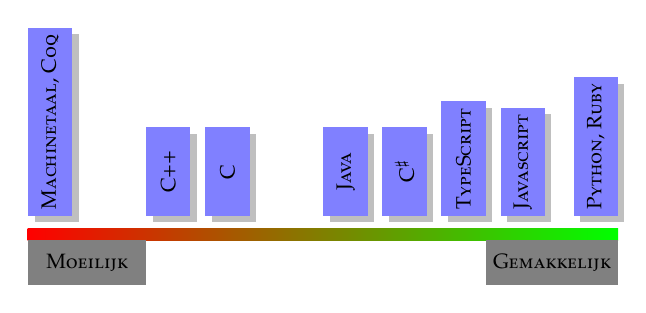
\begin{tikzpicture}[scale=.75,transform shape,
                        header/.style={fill=gray,minimum width=2cm,minimum height=0.75cm,font=\scshape}]
      \shade [left color=red,right color=green] (0,-0.4) rectangle (10,-0.2);
      
      \node[header,anchor=north west] at (0,-0.4) {Moeilijk};
      \node[header,anchor=north east] at (10,-0.4) {Gemakkelijk};

      \node[language,rotate=90,anchor=north west] at (0,0) {Machinetaal, Coq};
      \node[language,rotate=90,anchor=north west] at (3,0) {C};
      \node[language,rotate=90,anchor=north west] at (2,0) {\cpp};
      \node[language,rotate=90,anchor=north west] at (5,0) {Java};
      \node[language,rotate=90,anchor=north west] at (6,0) {\csharp};
      \node[language,rotate=90,anchor=north west] at (7,0) {TypeScript};
      \node[language,rotate=90,anchor=north west] at (8,0) {Javascript};
      \node[language,rotate=90,anchor=south west] at (10,0) {Python, Ruby};
    \end{tikzpicture}
  \end{center}
\end{frame}

\begin{frame}
  \frametitle{Teamwork}
  \begin{itemize}
    \item Sommige talen zijn enkel geschikt voor kleine teams
    \item Andere bieden ondersteuning voor grote teams
  \end{itemize}

  \begin{center}
    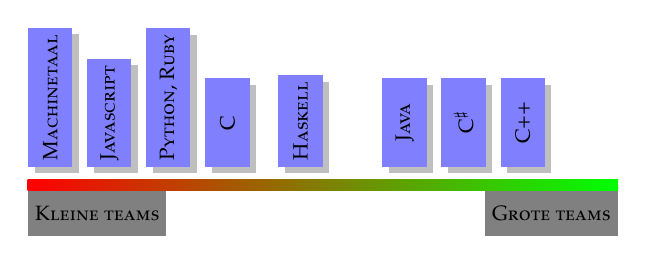
\begin{tikzpicture}[scale=.75,transform shape,
                        header/.style={fill=gray,minimum width=2cm,minimum height=0.75cm,font=\scshape}]
      \shade [left color=red,right color=green] (0,-0.4) rectangle (10,-0.2);
      
      \node[header,anchor=north west] at (0,-0.4) {Kleine teams};
      \node[header,anchor=north east] at (10,-0.4) {Grote teams};

      \node[language,rotate=90,anchor=north west] at (0,0) {Machinetaal};
      \node[language,rotate=90,anchor=north west] at (3,0) {C};
      \node[language,rotate=90,anchor=north west] at (8,0) {\cpp};
      \node[language,rotate=90,anchor=north west] at (7,0) {\csharp};
      \node[language,rotate=90,anchor=north west] at (6,0) {Java};
      \node[language,rotate=90,anchor=north west] at (2,0) {Python, Ruby};
      \node[language,rotate=90,anchor=north west] at (1,0) {Javascript};
      \node[language,rotate=90,anchor=south west] at (5,0) {Haskell};
    \end{tikzpicture}
  \end{center}
\end{frame}

\begin{frame}
  \frametitle{Low vs High Level}
  \begin{itemize}
    \item Sommige talen verbergen details van de machine
    \item Andere geven toegang tot de ``organen'' van de machine
  \end{itemize}

  \begin{center}
    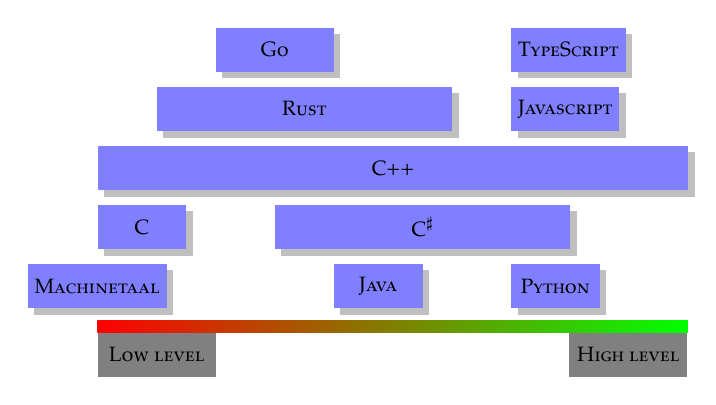
\begin{tikzpicture}[scale=.75,transform shape,
                        header/.style={fill=gray,minimum width=2cm,minimum height=0.75cm,font=\scshape}]
      \shade [left color=red,right color=green] (0,-0.4) rectangle (10,-0.2);
      
      \node[header,anchor=north west] at (0,-0.4) {Low level};
      \node[header,anchor=north east] at (10,-0.4) {High level};

      \node[language,anchor=south] at (0,0) {Machinetaal};
      \node[language,anchor=south west] at (0,1) {C};
      \node[language,anchor=south west,minimum width=10cm] at (0,2) {\cpp};
      \node[language,anchor=south west,minimum width=5cm] at (3,1) {\csharp};
      \node[language,anchor=south west] at (4,0) {Java};
      \node[language,anchor=south west] at (7,0) {Python};
      \node[language,anchor=south west] at (7,3) {Javascript};
      \node[language,anchor=south west,minimum width=5cm] at (1,3) {Rust};
      \node[language,anchor=south west] at (7,4) {TypeScript};
      \node[language,anchor=south west,minimum width=2cm] at (2,4) {Go};
    \end{tikzpicture}
  \end{center}
\end{frame}


%%% Local Variables:
%%% mode: latex
%%% TeX-master: "programming-languages"
%%% End:

\section{Talen}

\begin{frame}
  \tableofcontents[currentsection]
\end{frame}

\begin{frame}
  \frametitle{Machinetaal/Assembly}
  \structure{Kenmerken}
  \begin{itemize}
    \item Rock bottom level
    \item Potentieel heel effici\"ent
    \item Heel platformspecifiek
    \item Zo goed als geen libraries
  \end{itemize}
  \vskip4mm
  \structure{Toepassingen}
  \begin{itemize}
    \item Real-time systemen
    \item Low level embedded systems
    \item Drivers
  \end{itemize}
\end{frame}

\begin{frame}
  \frametitle{C}
  \structure{Kenmerken}
  \begin{itemize}
    \item Zeer low level: geeft quasi volledige controle over machine
    \item Zeer effici\"ent, maar onveilig in gebruik
  \end{itemize}
  \vskip4mm
  \structure{Toepassingen}
  \begin{itemize}
    \item Goed voor besturingssystemen
          \begin{itemize}
            \item Windows
            \item Linux
            \item Java VM
            \item Android
            \item iOS
          \end{itemize}
    \item Goed voor ``kleine'' machines
          \begin{itemize}
            \item Sensoren
            \item Autocomponenten
            \item Kredietkaartlezers
            \item \dots
          \end{itemize}
  \end{itemize}
\end{frame}

\begin{frame}
  \frametitle{\cpp}
  \structure{Kenmerken}
  \begin{itemize}
    \item Zowel low als high level
    \item Zeer gericht op effici\"entie
    \item Beetje veiliger dan C, maar nog steeds angstaanjagend
    \item Gericht naar teamontwikkeling
  \end{itemize}
  \vskip4mm
  \structure{Toepassingen}
  \begin{itemize}
    \item Spellen (Windows, PS, XBox, \dots)
    \item Meeste desktopapplicaties
    \item Complexe software die effici\"ent moet draaien
  \end{itemize}
\end{frame}

\begin{frame}
  \frametitle{Java, C\#}
  \structure{Kenmerken}
  \begin{itemize}
    \item Eerder high level
    \item 50-80\% effici\"entie van C/\cpp
    \item Ontwikkeld met veiligheid als doel
    \item Geen duidelijke specialisatie
    \item Gericht naar ontwikkeling in team
  \end{itemize}
  \vskip4mm
  \structure{Toepassingen}
  \begin{itemize}
    \item Server software
    \item GUI applicaties
    \item ``Lichte'' spellen (bv. Minecraft, Unity Engine)
  \end{itemize}
\end{frame}

\begin{frame}
  \frametitle{Python}
  \structure{Kenmerken}
  \begin{itemize}
    \item High level
    \item 10-20\% effici\"entie van C/\cpp
    \item Gebruiksgemak
    \item Gericht naar snelle ontwikkeling
    \item Ideaal voor kleine programma's
    \item Zeer breed toepassingsgebied
  \end{itemize}
  \vskip4mm
  \structure{Toepassingen}
  \begin{itemize}
    \item Automatisatie simpele taken
    \item Lichte spellen
    \item Eenvoudige GUI's
  \end{itemize}
\end{frame}

\begin{frame}
  \frametitle{Javascript}
  \structure{Kenmerken}
  \begin{itemize}
    \item Is in feite de ``machinetaal'' van het web
    \item Oorspronkelijk enkel bedoeld voor simpele taken
    \item Groei web heeft Javascript mee doen groeien
    \item Uitgebreid met ondersteuning complexe software
          \begin{itemize}
            \item Klassen
            \item Generators
          \end{itemize}
  \end{itemize}
  \vskip4mm
  \structure{Toepassingen}
  \begin{itemize}
    \item Quasi alles op het web
    \item NodeJS voor buiten de browser
  \end{itemize}
\end{frame}

\begin{frame}
  \frametitle{TypeScript}
  \structure{Kenmerken}
  \begin{itemize}
    \item Uitbreiding van Javascript
    \item Voert compile time checks in
          \begin{itemize}
            \item Enorme hulp bij ontwikkeling grotere programma's
          \end{itemize}
    \item Wordt vertaald naar Javascript
  \end{itemize}
  \vskip4mm
  \structure{Toepassingen}
  \begin{itemize}
    \item Zelfde als Javascript
  \end{itemize}
\end{frame}


%%% Local Variables:
%%% mode: latex
%%% TeX-master: "programming-languages"
%%% End:

\section{Curriculum}

\begin{frame}
  \tableofcontents[currentsection]
\end{frame}

\begin{frame}
  \frametitle{Curriculum}
  \begin{center}
    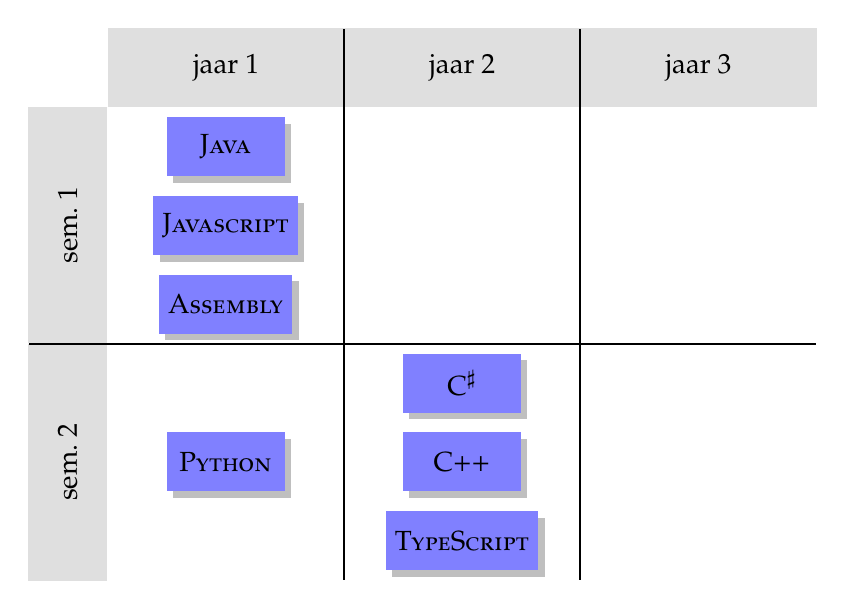
\begin{tikzpicture}[label/.style={fill=gray!25,minimum width=3cm,minimum height=1cm},
                        hlabel/.style={label},
                        vlabel/.style={label,rotate=90}]
      \node[vlabel,anchor=south west] at (0,0) {sem.~1};
      \node[vlabel,anchor=south east] at (0,0) {sem.~2};
      \node[hlabel,anchor=south west] at (0,3) {jaar 1};
      \node[hlabel,anchor=south west] at (3,3) {jaar 2};
      \node[hlabel,anchor=south west] at (6,3) {jaar 3};

      \draw[thick] (-1,0) -- (9,0);
      \draw[thick] (3,-3) -- (3,4);
      \draw[thick] (6,-3) -- (6,4);

      \node[language] at (1.5,2.5) {Java};
      \node[language] at (1.5,1.5) {Javascript};
      \node[language] at (1.5,0.5) {Assembly};

      \node[language] at (1.5,-1.5) {Python};

      \node[language] at (4.5,-0.5) {\csharp};
      \node[language] at (4.5,-1.5) {\cpp};
      \node[language] at (4.5,-2.5) {TypeScript};
    \end{tikzpicture}
  \end{center}
\end{frame}


%%% Local Variables:
%%% mode: latex
%%% TeX-master: "programming-languages"
%%% End:


\end{document}



%%% Local Variables: 
%%% mode: latex
%%% TeX-master: t
%%% End: 
